%%%%%%%%%%%%%%%%%%%%%%%%%%%%%%%%%%%%%%%%%%%%%%%%%%%%%%%%%%%%%%%%%%%%%%%%%%%%%%%
%% 1.- ESTADO DEL ARTE
%%%%%%%%%%%%%%%%%%%%%%%%%%%%%%%%%%%%%%%%%%%%%%%%%%%%%%%%%%%%%%%%%%%%%%%%%%%%%%%

\cleardoublepage
\chapter{Estado del arte}
\chaptermark{Estado del arte}

\label{chap:estadoArte} % etiqueta para poder referenciar luego en el texto con ~\ref{sec:intro}
% \addcontentsline{toc}{chapter}{Introducción, Objetivos, Metodología y Planificación}

El presente proyecto parte de un pedido realizado por un cliente que pretende comunicar con Kiconex los distintos equipos de un supermercado: muebles frigoríficos y máquinas de climatización. La mayoría de estos equipos dispone de un controlador propio, sin embargo, en el caso de la climatización, ha solicitado el diseño de un control a medida para el funcionamiento de una UTA. La instalación cuenta con los elementos de la \hyperref[figura:planoSupermercado]{Figura~\ref{figura:planoSupermercado}}:

\begin{figure}[h]
  \centering
  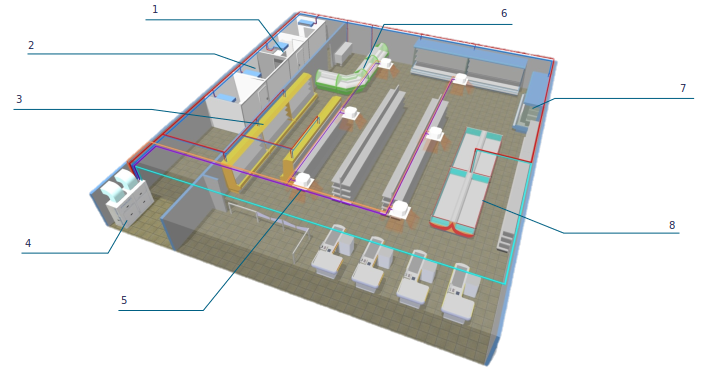
\includegraphics[width=16cm, keepaspectratio]{img/planoSupermercado}
  \caption{Plano de equipos del supermercado}
  \label{figura:planoSupermercado}
\end{figure}

\begin{enumerate}
  \item Obradores.
  \item Cámaras frigoríficas.
  \item Murales de lácteos.
  \item Bomba de calor.
  \item Unidades de Tratamiento de Aire.
  \item Vitrinas expositoras.
  \item Semimurales de carne, frutas y verduras.
  \item Islas de congelados.
\end{enumerate}

Kiconex emplea en sus desarrollos controladores de Dixell\footnote{\url{https://climate.emerson.com/es-es/brands/dixell}}, en concreto los modelos IPG208 e IPG215 de iPro\footnote{\url{https://climate.emerson.com/documents/ipro-series-en-4923358.pdf}}, con los módulos de expansión IPX206 e IPX215\footnote{\url{https://www.dixell-emerson.pl/upload/upload/Katalog/strony_katalogowe/CAT_GEN_13_GB_1.0%20iProGENIUS.pdf}}. El modelo a emplear dependerá de las especificaciones de entradas y salidas de la UTA que aparece en la \hyperref[figura:planoSupermercado]{Figura~\ref{figura:planoSupermercado}}. A continuación, en el \hyperref[sec:kiconex]{apartado 1 de este capítulo} se describe el software necesario para la programación de un control de este tipo.

El dispositivo inalámbrico a diseñar, mencionado en el \hyperref[chap:intro]{apartado de introducción anterior} comunicará los muebles frigoríficos: Murales de lácteos, vitrinas expositoras, semimurales e islas de congelados. El hardware empleado, descrito en el \hyperref[sec:esp32poe]{apartado 3 de este capítulo}, se basa en el chip ESP32\footnote{\url{https://www.espressif.com/en/products/socs/esp32/overview}}. Para entender el papel de este dispositivo en la red, es necesario conocer el funcionamiento de una instalación desde el punto de vista de Kiconex, atendiendo a cómo se integra cada elemento. El \hyperref[sec:kiconex]{apartado 2 de este capítulo} se dedica por completo a describir la estructura de un sistema basado en Kiconex.

\section{iPro y su pantalla}
\label{sec:iproypantalla}

\begin{figure}[h]
  \centering
  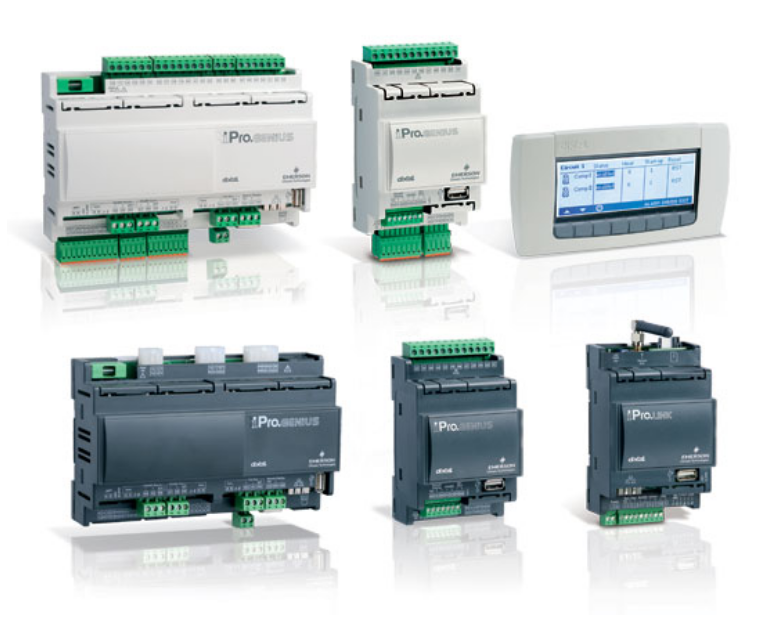
\includegraphics[width=12cm, keepaspectratio]{img/iproSeries}
  \caption{iPro Series}
  \label{figura:iproSeries}
\end{figure}

iPro (\hyperref[figura:iproSeries]{Figura~\ref{figura:iproSeries}}) es la gama de controladores programables ofrecida por Dixell. La gama consta de controladores programables, ampliaciones de E/S, controladores para válvulas electrónicas e interfaces gráficas adaptadas para cubrir cualquier tipo de aplicación en el sector del aire acondicionado, el sector de la refrigeración y cualquier área relativa. Algunas de sus especificaciones son:

\begin{itemize}
  \item Alimentación a 24Vac/dc.
  \item Microprocesador ARM9 de 32 bits (200MHz).
  \item El programa y los parámetros se almacenan en una memoria flash permanente. No se pierden datos en caso de fallo de alimentación.
  \item Servidor web interno.
  \item Hasta 80 Mb de memoria flash, dependiendo del modelo.
  \item Entradas y salidas completamente configurables.
  \item Conexiones:
  \begin{itemize}
    \item Puerto Ethernet.
    \item Puerto USB.
    \item Conexión dedicada para un display LCD.
    \item CANBus.
    \item RS485 Master.
    \item RS485 Slave.
  \end{itemize}
\end{itemize}

Los modelos se diferencian en el tamaño (10 DIN o 4 DIN) y en el número de entradas y salidas (analógicas y digitales). La \hyperref[tab:esipro]{Tabla~\ref{tab:esipro}} recoge las especificaciones de los modelos empleados por Kiconex.

\begin{table}[h]
  %\centering
  \begin{center}
    \setlength\arrayrulewidth{2pt}
    \begin{tabular}{ r | c !{\vrule width 0.25pt} c | c !{\vrule width 0.25pt} c | }
      %\Cline{2pt}{2-5}
      \hhline{*{1}{~}|*{4}{-}}
      \multirow{2}{*} & \multicolumn{2}{c|}{\cellcolor{lightgray}Controlador} & \multicolumn{2}{c|}{\cellcolor{lightgray}Módulo de Expansión}   \\ \Cline{0.25pt}{2-5}
      & \textbf{IPG208} & \textbf{IPG215} & \textbf{IPX206} & \textbf{IPX215} \\ \cline{1-1} \Cline{0.25pt}{2-5}
      \multicolumn{1}{|r|}{\textbf{Entradas analógicas}} & 6 & 10 & 7 & 10 \\
      \multicolumn{1}{|r|}{\textbf{Salidas analógicas}} & 4 & 6 & 3 & 6 \\
      \multicolumn{1}{|r|}{\textbf{Entradas digitales}} & 11 & 20 & 3 & 20 \\
      \multicolumn{1}{|r|}{\textbf{Salidas digitales (Relés)}} & 8 & 6 & 8 & 15 \\ 
      \noalign{\hrule height 2pt}
    \end{tabular}
    \caption{Especificaciones de E/S para distintos modelos de iPro.}
    \label{tab:esipro}
  \end{center}
\end{table} 

Dixell dispone de dos modelos de displays compatibles con el iPro: VGIPG y VTIPG\footnote{\url{https://climate.emerson.com/es-es/shop/1/dixell-electronics-sku-vtipg-hmi-es-es}}. Para el diseño de dichas pantallas, se emplea el software VISOPROG\footnote{\url{https://climate.emerson.com/es-es/shop/1/dixell-electronics-sku-visoprog-es-es}} de Dixell, que importa las variables creadas en la programación del controlador, para poder configurar en la pantalla la interacción con las mismas. 

\subsection{Programación iPro}
\label{subsec:iproprog}

Para la programación del iPro se emplea un software 

\subsection{Configuración de la pantalla}
\label{subsec:displayconfig}

Para la configuración de la pantalla, se emplea Visoprog, un software ofrecido por la misma marca Dixell.


\section{Kiconex}
\label{sec:kiconex}

asdfasdf

\section{ESP32-PoE}
\label{sec:esp32poe}
assada

%%%%%%%%%%%%%%%%%%%%%%%%%%%%%%%%%%%%%%%%%%%%%%%%%%%%%%%%%%%%%%%%%%%%%%%%%%%%%%%
%%%%%%%%%%%%%%%%%%%%%%%%%%%%%%%%%%%%%%%%%%%%%%%%%%%%%%%%%%%%%%%%%%%%%%%%%%%%%%%
%%%%%%%%%%%%%%%%%%%%%%%%%%%%%%%%%%%%%%%%%%%%%%%%%%%%%%%%%%%%%%%%%%%%%%%%%%%%%%%
